%!TEX root = ../slides.tex
\section{Theoretical framework}
\subsection{Stay points}
\begin{frame}{Theoretical framework}{Stay points, Event Driven Systems (EDSs)}
\small
\begin{block}{\small \textbf{Stay point}}
\begin{itemize}
  \item A stay point refers to a geographical zone (of size $\delta_{distance}$) where the user remains for an amount of time ($\delta_{time}$).
  \item It is a virtual location defined by latitude (\emph{lat}), longitude (\emph{lon}), arrival time (\emph{at}) and departure time (\emph{dt}).
\end{itemize}
\end{block}

\begin{block}{\small \textbf{Event Driven Systems (EDSs)}}
{
    \centering
    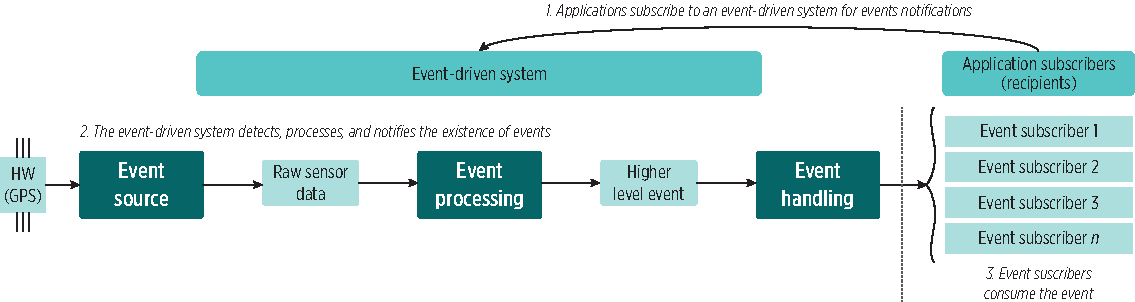
\includegraphics[width=0.85\textwidth]{vectors/event-driven-system-for-slides}
    \captionof{figure}{The architecture of an EDS.}
    \par
}
% \begin{itemize}
%   \item An event is an occurrence within a particular system-domain~\cite{Etzion2011} at an specific timestamp or during a time interval.
%   \item An EDS is a system that works by sending asynchronous event notifications between its components for triggering computing tasks~\cite{Etzion2011,Faison2011}.
% \end{itemize}
\end{block}

% \begin{block}{\small \textbf{Cognitive Dynamic Systems (CDSs)}}
% \begin{figure}
%     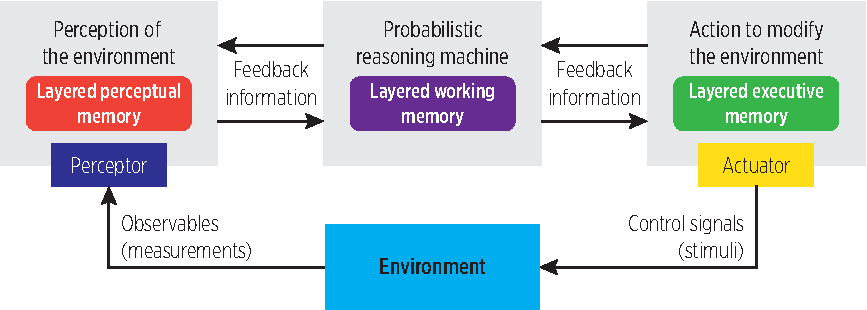
\includegraphics[width=0.6\textwidth]{vectors/cds-adaptation-figure-for-slides}
%     \caption{The generic architecture of a CDS.}
% \end{figure}
% \end{block}

% \begin{block}{\small \textbf{Event Driven System (EDS)}}
% \begin{itemize}
%   \item An EDS is a system that works by sending asynchronous event notifications between its components for triggering computing tasks~\cite{Faison2011,Etzion2011}.
%   \item Its complexity and coupling is reduced and it is power-aware by design (vs. synchronous systems~\cite{Rawassizadeh2015,Lee2015,Duffy2007}).
% \end{itemize}
% \end{block}

% {
%     \centering
%     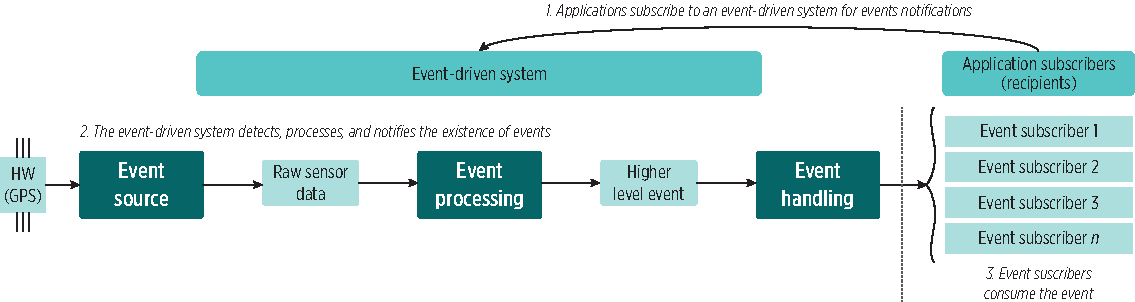
\includegraphics[width=0.9\textwidth]{vectors/event-driven-system-for-slides}
%     \captionof{figure}{The architecture of an EDS.}
%     \par
% }

% \begin{block}{\small \textbf{Calculation}}
% \begin{itemize}
%   \item A GPS position fix $p$ is defined by latitude ($lat$), longitude ($lon$), and timestamp ($t$).

%   \item A stay point ($\mathbf{sp}$) is calculated from a set of consecutive GPS fixes $\mathbf{P}=\{p_{m},p_{m+1},\ldots,p_{n}\}$, and $\delta_{distance}$ and $\delta_{time}$ thresholds. 
  
%   \item Its composition must observe:
%   \begin{columns}
%   \begin{column}{0.5\textwidth}
%   \begin{equation*}
%     \left|p_{n}.t-p_{m}.t\right|\geq\delta_{time}
%   \end{equation*}
%   \end{column}

%   \begin{column}{0.5\textwidth}
%   \begin{equation*}
%     \text{distance}(p_{m},p_{i})\leq\delta_{distance}, \forall m<i\leq n
%   \end{equation*}
%   \end{column}
%   \end{columns}
  
%   \item Its centroid coordinates are the arithmetical means:
%   \begin{columns}
%   \begin{column}{0.5\textwidth}
%   \begin{equation*}
%   \mathbf{sp}.lat = \frac{ \sum_{i=m}^{n}p_{i}.lat }{ |\mathbf{P}| }\label{eq:centroid-latitude}
%   \end{equation*}
%   \end{column}

%   \begin{column}{0.5\textwidth}
%   \begin{equation*}
%   \mathbf{sp}.lon = \frac{ \sum_{i=m}^{n}p_{i}.lon }{ |\mathbf{P}| }\label{eq:centroid-longitude}
%   \end{equation*}
%   \end{column}
%   \end{columns}
%   \item The \emph{at} and \emph{dt} components are set to $p_m.t$ and $p_n.t$, respectively.
% \end{itemize}
% \end{block}
\end{frame}

% \subsection{Event Driven Systems}
% \begin{frame}{Theoretical framework}{Event Driven Systems (EDSs)}
% \small
% \vspace{-0.2cm}
% \begin{block}{\small \textbf{Event}}
% \begin{itemize}
%   % \item It is an occurrence within a particular system-domain; it is something that has happened in that domain~\cite{Etzion2011}.
%   \item It is an occurrence within a particular system-domain~\cite{Etzion2011} at an specific timestamp or during a time interval.
%   \item Formally defined as:
%   \begin{equation*}
%     ev = ev(id, \left\{ a_1,a_2,\ldots, a_n \right\}, t)
%   \end{equation*}
%   where $id$ is an identifier, $\left\{ a_1,a_2,\ldots, a_n \right\}$ is a list of $n$ associated attributes, and $t$ the timestamp.
% \end{itemize}
% \end{block}

% \begin{block}{\small \textbf{Event Driven System (EDS)}}
% \begin{itemize}
%   \item An EDS is a system that works by sending asynchronous event notifications between its components for triggering computing tasks~\cite{Faison2011,Etzion2011}.
%   \item Its complexity and coupling is reduced and it is power-aware by design (vs. synchronous systems~\cite{Rawassizadeh2015,Lee2015,Duffy2007}).
% \end{itemize}
% \end{block}

% {
%     \centering
%     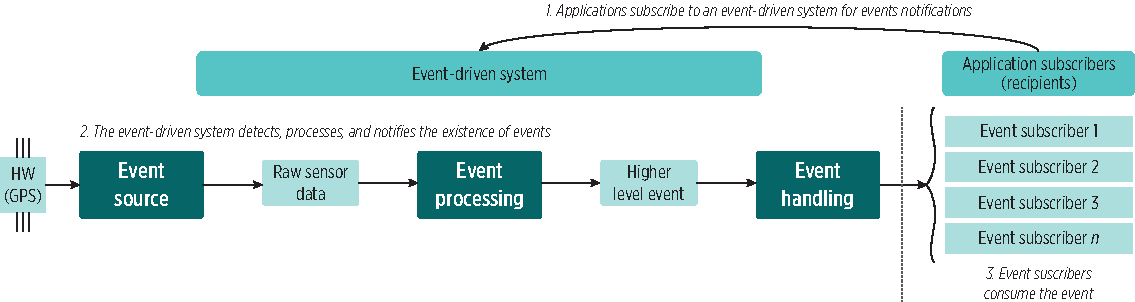
\includegraphics[width=0.9\textwidth]{vectors/event-driven-system-for-slides}
%     \captionof{figure}{The architecture of an EDS.}
%     \par
% }
% \end{frame}


\subsection{Cognitive Dynamic Systems}
\begin{frame}{Theoretical framework}{Cognitive Dynamic Systems (CDSs)}
\small
\vspace{-0.2cm}
% \begin{block}{\small \textbf{Features}}
% \begin{itemize}
%   \item Perception-action cycle
%   \item Memory
%   \item Attention
%   \item Intelligence
% \end{itemize}
% \end{block}

% \begin{column}[T]{0.8\textwidth}

\begin{block}{\small \textbf{Features}}
% \begin{columns}
% \begin{column}[T]{0.3\textwidth}
\begin{itemize}
  \item Perception-action cycle
% \end{itemize}
% \end{column}

% \begin{column}[T]{0.2\textwidth}
% \begin{itemize}
  \item Memory
% \end{itemize}
% \end{column}

% \begin{column}[T]{0.2\textwidth}
% \begin{itemize}
  \item Attention
% \end{itemize}
% \end{column}

% \begin{column}[T]{0.2\textwidth}
% \begin{itemize}
  \item Intelligence
\end{itemize}
% \end{column}

% \end{columns}

\end{block}

\begin{figure}
    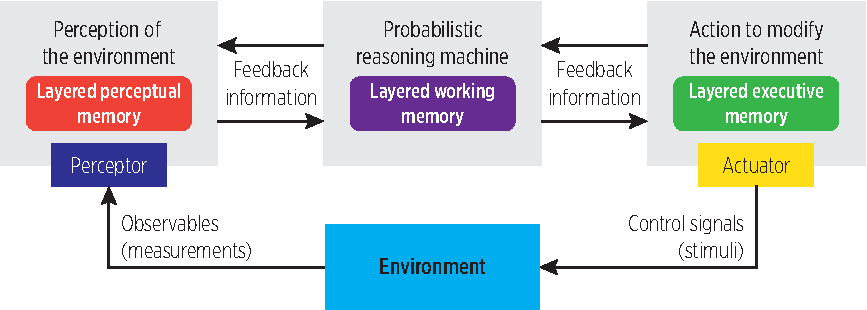
\includegraphics[width=0.6\textwidth]{vectors/cds-adaptation-figure-for-slides}
    \caption{The generic architecture of a CDS.}
\end{figure}


\end{frame}
